\documentclass{beamer}
\usepackage[utf8]{inputenc}
\usepackage{amsmath}

\usetheme{Boadilla}

\title{The Dynare Macro-processor}
\subtitle{Dynare Summer School 2013}
\author{Sébastien Villemot}
\institute{CEPREMAP}
\date{June 28, 2013}

\AtBeginSection[]
{
  \begin{frame}
    \frametitle{Outline}
    \tableofcontents[currentsection]
  \end{frame}
}

\begin{document}

\begin{frame}
  \titlepage
\end{frame}

\begin{frame}
  \frametitle{Outline}
  \tableofcontents
\end{frame}

\section{Overview}

\begin{frame}
  \frametitle{Motivation}
  \begin{itemize}
  \item The \textbf{Dynare language} (used in MOD files) is well suited for many economic models
  \item However, as such, it lacks some useful features, such as:
    \begin{itemize}
    \item a loop mechanism for automatically repeating similar blocks of equations (such as in multi-country models)
    \item an operator for indexed sums or products inside equations
    \item a mechanism for splitting large MOD files in smaller modular files
    \item the possibility of conditionally including some equations or some runtime commands
  \end{itemize}
  \item The \textbf{Dynare Macro-language} was specifically designed to address these issues
  \item Being flexible and fairly general, it can also be helpful in other situations
  \end{itemize}
\end{frame}

\begin{frame}
  \frametitle{Design of the macro-language}
  \begin{itemize}
  \item The Dynare Macro-language provides a new set of \textbf{macro-commands} which can be inserted inside MOD files
  \item Language features include:
    \begin{itemize}
    \item file inclusion
    \item loops (\textit{for} structure)
    \item conditional inclusion (\textit{if/else} structures)
    \item expression substitution
    \end{itemize}
  \item Implemented in Dynare starting from version 4.0
  \item The macro-processor transforms a MOD file with macro-commands into a MOD file without macro-commands (doing text expansions/inclusions) and then feeds it to the Dynare parser
  \item The key point to understand is that the macro-processor only does \textbf{text substitution} (like the C preprocessor or the PHP language)
  \end{itemize}
\end{frame}

\begin{frame}
  \frametitle{Design of Dynare}
  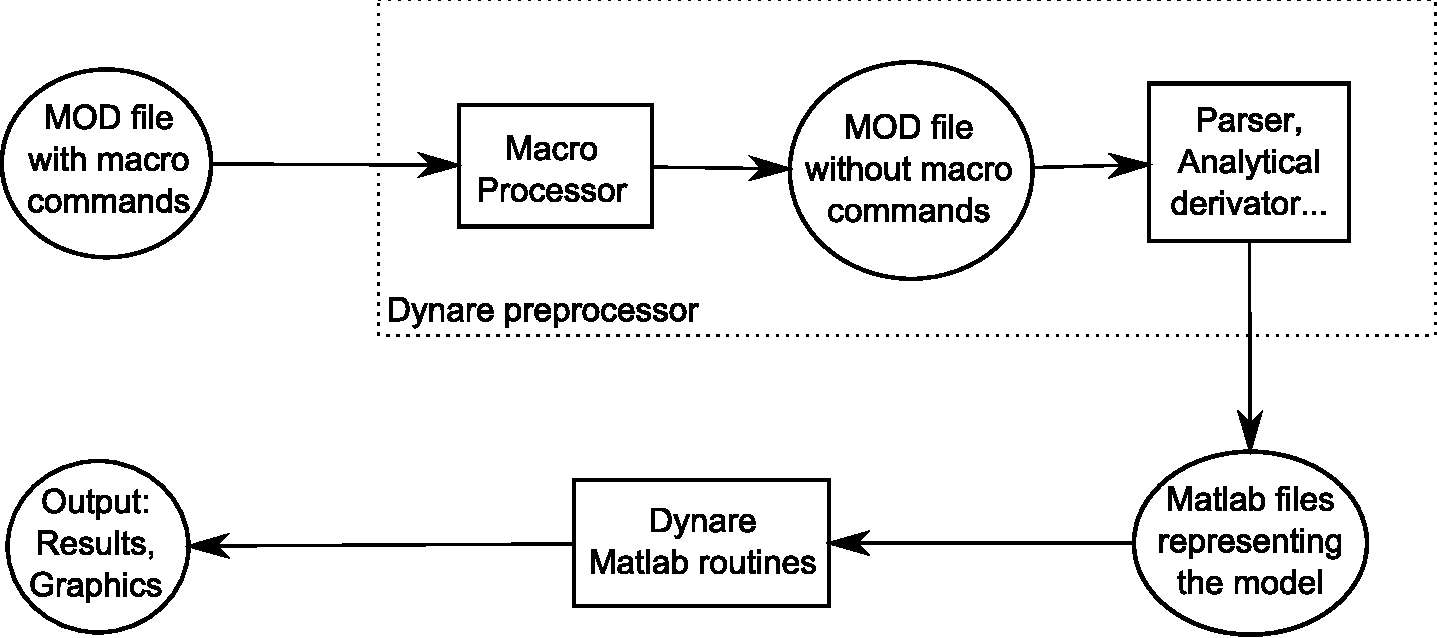
\includegraphics[width=0.95\linewidth]{new-design.pdf}
\end{frame}

\section{Syntax}

\begin{frame}[fragile=singleslide]
  \frametitle{Macro Directives}
  \begin{itemize}
  \item Directives begin with an at-sign followed by a pound sign (\verb+@#+)
  \item A directive produces no output, but gives instructions to the macro-processor
  \item Main directives are:
    \begin{itemize}
    \item file inclusion: \verb+@#include+
    \item definition a variable of the macro-processor: \verb+@#define+
    \item conditional statements (\verb+@#if/@#ifdef/@#ifndef/@#else/@#endif+)
    \item loop statements (\verb+@#for/@#endfor+)
    \end{itemize}
  \item In most cases, directives occupy exactly one line of text. In case of need, two anti-slashes (\verb+\\+) at the end of the line indicates that the directive is continued on the next line.
  \end{itemize}
\end{frame}

\begin{frame}[fragile=singleslide]
  \frametitle{Inclusion directive}
  \begin{itemize}
  \item This directive simply includes the content of another file at the place where it is inserted.
    \begin{block}{Syntax}
      \verb+@#include "+\textit{filename}\verb+"+
    \end{block}
    \begin{block}{Example}
\begin{verbatim}
@#include "modelcomponent.mod"
\end{verbatim}
    \end{block}
  \item Exactly equivalent to a copy/paste of the content of the included file
  \item Note that it is possible to nest includes (\textit{i.e.} to include a file from an included file)
  \end{itemize}
\end{frame}

\begin{frame}
\frametitle{Variables}
\begin{itemize}
\item The macro processor maintains its own list of variables (distinct of model variables and of MATLAB variables)
\item Macro-variables can be of four types:
  \begin{itemize}
  \item integer
  \item character string (declared between \textit{double} quotes)
  \item array of integers
  \item array of strings
  \end{itemize}
\item No boolean type:
  \begin{itemize}
  \item false is represented by integer zero
  \item true is any non-null integer
  \end{itemize}
\end{itemize}
\end{frame}

\begin{frame}[fragile=singleslide]
  \frametitle{Macro-expressions (1/2)}
  It is possible to construct macro-expressions, using standard operators.
  \begin{block}{Operators on integers}
    \begin{itemize}
    \item arithmetic operators: \texttt{+ - * /}
    \item comparison operators: \texttt{< > <= >= == !=}
    \item logical operators: \verb+&& || !+
    \item integer ranges: \texttt{1:4} is equivalent to integer array \texttt{[1,2,3,4]}
    \end{itemize}
  \end{block}

  \begin{block}{Operators on character strings}
    \begin{itemize}
    \item comparison operators: \texttt{== !=}
    \item concatenation: \texttt{+}
    \item extraction of substrings: if \texttt{s} is a string, then one can write \texttt{s[3]} or \texttt{s[4:6]}
    \end{itemize}
  \end{block}
\end{frame}

\begin{frame}[fragile=singleslide]
  \frametitle{Macro-expressions (2/2)}
  \begin{block}{Operators on arrays}
    \begin{itemize}
    \item dereferencing: if \texttt{v} is an array, then \texttt{v[2]} is its $2^{\textrm{nd}}$ element
    \item concatenation: \texttt{+}
    \item difference \texttt{-}: returns the first operand from which the elements of the second operand have been removed
    \item extraction of sub-arrays: \textit{e.g.} \texttt{v[4:6]}
    \item testing membership of an array: \texttt{in} operator \\ (example:
      \texttt{"b" in ["a", "b", "c"]} returns \texttt{1})
    \end{itemize}
  \end{block}

  Macro-expressions can be used at two places:
  \begin{itemize}
  \item inside macro directives, directly
  \item in the body of the MOD file, between an at-sign and curly braces (like \verb+@{expr}+): the macro processor will substitute the expression with its value
  \end{itemize}
\end{frame}

\begin{frame}[fragile=singleslide]
  \frametitle{Define directive}

  The value of a macro-variable can be defined with the \verb+@#define+ directive.

  \begin{block}{Syntax}
    \verb+@#define +\textit{variable\_name}\verb+ = +\textit{expression}
  \end{block}

  \begin{block}{Examples}
\begin{verbatim}
@#define x = 5              // Integer
@#define y = "US"           // String
@#define v = [ 1, 2, 4 ]    // Integer array
@#define w = [ "US", "EA" ] // String array
@#define z = 3 + v[2]       // Equals 5
@#define t = ("US" in w)    // Equals 1 (true)
\end{verbatim}
  \end{block}
\end{frame}

\begin{frame}[fragile=singleslide]
  \frametitle{Expression substitution}
  \framesubtitle{Dummy example}
  \begin{block}{Before macro-processing}
\begin{verbatim}
@#define x = [ "B", "C" ]
@#define i = 2

model;
  A = @{x[i]};
end;
\end{verbatim}
  \end{block}
  \begin{block}{After macro-processing}
\begin{verbatim}
model;
  A = C;
end;
\end{verbatim}
  \end{block}
\end{frame}

\begin{frame}[fragile=singleslide]
  \frametitle{Loop directive}
  \begin{block}{Syntax}
\verb+@#for +\textit{variable\_name}\verb+ in +\textit{array\_expr} \\
\verb+   +\textit{loop\_body} \\
\verb+@#endfor+
  \end{block}
  \begin{block}{Example: before macro-processing}
    \small
\begin{verbatim}
model;
@#for country in [ "home", "foreign" ]
  GDP_@{country} = A * K_@{country}^a * L_@{country}^(1-a);
@#endfor
end;
\end{verbatim}
    \normalsize
  \end{block}

  \begin{block}{Example: after macro-processing}
    \small
\begin{verbatim}
model;
  GDP_home = A * K_home^a * L_home^(1-a);
  GDP_foreign = A * K_foreign^a * L_foreign^(1-a);
end;
\end{verbatim}
    \normalsize
  \end{block}
\end{frame}

\begin{frame}[fragile=singleslide]
  \frametitle{Conditional inclusion directives (1/2)}

  \begin{columns}[T]
    \column{0.47\linewidth}
    \begin{block}{Syntax 1}
\verb+@#if +\textit{integer\_expr} \\
\verb+   +\textit{body included if expr != 0} \\
\verb+@#endif+
    \end{block}

    \column{0.47\linewidth}
    \begin{block}{Syntax 2}
\verb+@#if +\textit{integer\_expr} \\
\verb+   +\textit{body included if expr != 0} \\
\verb+@#else+ \\
\verb+   +\textit{body included if expr == 0} \\
\verb+@#endif+
    \end{block}
  \end{columns}

  \begin{block}{Example: alternative monetary policy rules}
    \scriptsize
\begin{verbatim}
@#define linear_mon_pol = 0 // or 1
...
model;
@#if linear_mon_pol
  i = w*i(-1) + (1-w)*i_ss + w2*(pie-piestar);
@#else
  i = i(-1)^w * i_ss^(1-w) * (pie/piestar)^w2;
@#endif
...
end;
\end{verbatim}
    \scriptsize
  \end{block}
\end{frame}

\begin{frame}[fragile=singleslide]
  \frametitle{Conditional inclusion directives (2/2)}

  \begin{columns}[T]
    \column{0.47\linewidth}
    \begin{block}{Syntax 1}
\verb+@#ifdef +\textit{variable\_name} \\
\verb+   +\textit{body included if variable defined} \\
\verb+@#endif+
    \end{block}

    \column{0.47\linewidth}
    \begin{block}{Syntax 2}
\verb+@#ifdef +\textit{variable\_name} \\
\verb+   +\textit{body included if variable defined} \\
\verb+@#else+ \\
\verb+   +\textit{body included if variable not defined} \\
\verb+@#endif+
    \end{block}
  \end{columns}

\bigskip

There is also \verb+@#ifndef+, which is the opposite of \verb+@#ifdef+
(\textit{i.e.} it tests whether a variable is \emph{not} defined).
\end{frame}

\begin{frame}[fragile=singleslide]
  \frametitle{Echo and error directives}

  \begin{itemize}
  \item The echo directive will simply display a message on standard output
  \item The error directive will display the message and make Dynare stop (only makes sense inside a conditional inclusion directive)
  \end{itemize}

  \begin{block}{Syntax}
\verb+@#echo +\textit{string\_expr} \\
\verb+@#error +\textit{string\_expr}
  \end{block}

  \begin{block}{Examples}
\begin{verbatim}
@#echo "Information message."
@#error "Error message!"
\end{verbatim}
  \end{block}
\end{frame}

\begin{frame}
  \frametitle{Saving the macro-expanded MOD file}
  \begin{itemize}
  \item For \textbf{debugging or learning} purposes, it is possible to save the output of the macro-processor
  \item This output is a valid MOD file, obtained after processing the macro-commands of the original MOD file
%  \item Useful to understand how the macro-processor works
  \item Just add the \texttt{savemacro} option on the Dynare command line (after the name of your MOD file)
  \item If MOD file is \texttt{filename.mod}, then the macro-expanded version will be saved in \texttt{filename-macroexp.mod}
  \item You can specify the filename for the macro-expanded version with the syntax \texttt{savemacro=mymacroexp.mod}
  \end{itemize}
\end{frame}

% \begin{frame}
%   \frametitle{Note on error messages}
% \end{frame}

\section{Typical usages}

\begin{frame}[fragile=singleslide]
  \frametitle{Modularization}
  \begin{itemize}
  \item The \verb+@#include+ directive can be used to split MOD files into several modular components
  \item Example setup:
    \begin{description}
    \item[\texttt{modeldesc.mod}:] contains variable declarations, model equations and shocks declarations
    \item[\texttt{simulate.mod}:] includes \texttt{modeldesc.mod}, calibrates parameters and runs stochastic simulations
    \item[\texttt{estim.mod}:] includes \texttt{modeldesc.mod}, declares priors on parameters and runs bayesian estimation
    \end{description}
  \item Dynare can be called on \texttt{simulate.mod} and \texttt{estim.mod}
  \item But it makes no sense to run it on \texttt{modeldesc.mod}
  \item Advantage: no need to manually copy/paste the whole model (at the beginning) or changes to the model (during development)
  \end{itemize}
\end{frame}

\begin{frame}[fragile=singleslide]
  \frametitle{Indexed sums or products}
  \framesubtitle{Example: moving average}
  \begin{columns}[T]
    \column{0.47\linewidth}
    \begin{block}{Before macro-processing}
\begin{verbatim}
@#define window = 2

var x MA_x;
...
model;
...
MA_x = 1/@{2*window+1}*(
@#for i in -window:window
        +x(@{i})
@#endfor
       );
...
end;
\end{verbatim}
    \end{block}
    \column{0.47\linewidth}
    \begin{block}{After macro-processing}
\begin{verbatim}
var x MA_x;
...
model;
...
MA_x = 1/5*(
        +x(-2)
        +x(-1)
        +x(0)
        +x(1)
        +x(2)
       );
...
end;
\end{verbatim}
    \end{block}
  \end{columns}
\end{frame}

\begin{frame}[fragile=singleslide]
  \frametitle{Multi-country models}
  \framesubtitle{MOD file skeleton example}
  \scriptsize
\begin{verbatim}
@#define countries = [ "US", "EA", "AS", "JP", "RC" ]
@#define nth_co = "US"

@#for co in countries
var Y_@{co} K_@{co} L_@{co} i_@{co} E_@{co} ...;
parameters a_@{co} ...;
varexo ...;
@#endfor

model;
@#for co in countries
 Y_@{co} = K_@{co}^a_@{co} * L_@{co}^(1-a_@{co});
...
@# if co != nth_co
 (1+i_@{co}) = (1+i_@{nth_co}) * E_@{co}(+1) / E_@{co}; // UIP relation
@# else
 E_@{co} = 1;
@# endif
@#endfor
end;
\end{verbatim}
  \normalsize
\end{frame}

\begin{frame}
  \frametitle{Endogeneizing parameters (1/4)}
  \begin{itemize}
  \item When doing the steady-state calibration of the model, it may be useful to consider a parameter as an endogenous (and vice-versa)
  \item Example:
    \begin{gather*}
      y = \left(\alpha^{\frac{1}{\xi}} \ell^{1-\frac{1}{\xi}} + (1-\alpha)^{\frac{1}{\xi}}k^{1-\frac{1}{\xi}}\right)^{\frac{\xi}{\xi - 1}} \\
      lab\_rat = \frac{w \ell}{p y}
    \end{gather*}
  \item In the model, $\alpha$ is a (share) parameter, and $lab\_rat$ is an endogenous variable
  \item We observe that:
    \begin{itemize}
    \item calibrating $\alpha$ is not straigthforward!
    \item on the contrary, we have real world data for $lab\_rat$
    \item it is clear that these two variables are economically linked
    \end{itemize}
  \end{itemize}
\end{frame}

\begin{frame}[fragile=singleslide]
  \frametitle{Endogeneizing parameters (2/4)}
  \begin{itemize}
  \item Therefore, when computing the steady state:
    \begin{itemize}
    \item we make $\alpha$ an endogenous variable and $lab\_rat$ a parameter
    \item we impose an economically relevant value for $lab\_rat$
    \item the solution algorithm deduces the implied value for $\alpha$
    \end{itemize}
  \item We call this method ``variable flipping''
  \end{itemize}
\end{frame}

\begin{frame}[fragile=singleslide]
  \frametitle{Endogeneizing parameters (3/4)}
  \framesubtitle{Example implementation}
  \begin{itemize}
  \item File \texttt{modeqs.mod}:
    \begin{itemize}
    \item contains variable declarations and model equations
    \item For declaration of \texttt{alpha} and \texttt{lab\_rat}:
    \footnotesize
\begin{verbatim}
@#if steady
 var alpha;
 parameter lab_rat;
@#else
 parameter alpha;
 var lab_rat;
@#endif
\end{verbatim}
    \normalsize
    \end{itemize}

  \end{itemize}
\end{frame}

\begin{frame}[fragile=singleslide]
  \frametitle{Endogeneizing parameters (4/4)}
  \framesubtitle{Example implementation}
  \begin{itemize}
  \item File \texttt{steadystate.mod}:
    \begin{itemize}
    \item begins with \verb+@#define steady = 1+
    \item then with \verb+@#include "modeqs.mod"+
    \item initializes parameters (including \texttt{lab\_rat}, excluding \texttt{alpha})
    \item computes steady state (using guess values for endogenous, including \texttt{alpha})
    \item saves values of parameters and endogenous at steady-state in a file, using the \texttt{save\_params\_and\_steady\_state} command
    \end{itemize}
  \item File \texttt{simulate.mod}:
    \begin{itemize}
    \item begins with \verb+@#define steady = 0+
    \item then with \verb+@#include "modeqs.mod"+
    \item loads values of parameters and endogenous at steady-state from file, using the \texttt{load\_params\_and\_steady\_state} command
    \item computes simulations
    \end{itemize}
  \end{itemize}
\end{frame}

\begin{frame}[fragile=singleslide]
  \frametitle{MATLAB loops vs macro-processor loops (1/3)}
  Suppose you have a model with a parameter $\rho$, and you want to make
  simulations for three values: $\rho = 0.8, 0.9, 1$. There are
  several ways of doing this:
  \begin{block}{With a MATLAB loop}
\begin{verbatim}
rhos = [ 0.8, 0.9, 1];
for i = 1:length(rhos)
  rho = rhos(i);
  stoch_simul(order=1);
end
\end{verbatim}
  \end{block}
  \begin{itemize}
  \item The loop is not unrolled
  \item MATLAB manages the iterations
  \item Interesting when there are a lot of iterations
  \end{itemize}
\end{frame}

\begin{frame}[fragile=singleslide]
  \frametitle{MATLAB loops vs macro-processor loops (2/3)}
  \begin{block}{With a macro-processor loop (case 1)}
\begin{verbatim}
rhos = [ 0.8, 0.9, 1];
@#for i in 1:3
  rho = rhos(@{i});
  stoch_simul(order=1);
@#endfor
\end{verbatim}
  \end{block}
  \begin{itemize}
  \item Very similar to previous example
  \item Loop is unrolled
  \item Dynare macro-processor manages the loop index but not the data array (\texttt{rhos})
  \end{itemize}
\end{frame}

\begin{frame}[fragile=singleslide]
  \frametitle{MATLAB loops vs macro-processor loops (3/3)}
  \begin{block}{With a macro-processor loop (case 2)}
\begin{verbatim}
@#for rho_val in [ "0.8", "0.9", "1"]
  rho = @{rho_val};
  stoch_simul(order=1);
@#endfor
\end{verbatim}
  \end{block}
  \begin{itemize}
  \item Advantage: shorter syntax, since list of values directly given in the loop construct
  \item Note that values are given as character strings (the macro-processor does not
    know floating point values)
  \item Inconvenient: can not reuse an array stored in a MATLAB variable
  \end{itemize}
\end{frame}

% \begin{frame}[fragile=singleslide]
%   \frametitle{Possible future developments}
%   \begin{itemize}
%   \item Find a nicer syntax for indexed sums/products
%   \item Implement other control structures: \texttt{elsif}, \texttt{switch/case}, \texttt{while/until} loops
%   \item Implement macro-functions (or templates), with a syntax like:
%     \small
%     \verb+@#define QUADRATIC_COST(x, x_ss, phi) = phi/2*(x/x_ss-1)^2+
%     \normalsize
%   \end{itemize}
% \end{frame}

\end{document}
